\documentclass{article}

% Lenguaje y Fuente
\usepackage[spanish]{babel}
\usepackage[utf8x]{inputenc}
\usepackage[T1]{fontenc}
\usepackage[top=1in, bottom=1.25in, left=1.1 in, right=1.1 in]{geometry}
\usepackage{graphicx}
\usepackage{ragged2e}
\usepackage[usenames]{color}
\usepackage{multicol}

% Portada

\title{\textbf{Reporte de la Actividad 7}\\ Visualización de datos con la biblioteca Seaborn}
\author{Luis Fernando Duarte Gonzalí \\ Universidad de Sonora \\ Física Computacional}
\date{Marzo del 2019}
\begin{document}
\maketitle

% Contenido del Reporte

\section{Introducción}
\subsection{Seaborn}
Seaborn es una librería de visualización de datos de Python basado en matplotlib. Provee una interfaz de alto nivel para dibujar gráficas estadísticas atractivas e informativas.

Seaborn tiene como objetivo el hacer la visualización una parte central de exploración y entendimiento de datos. Sus funciones para graficar orientadas en datasets operan en \textit{Dataframes} y arreglos que contienen datasets completos e internamente desarrollan la semántica de mapeos y agregación estadística necesaria para producir gráficas informativas.

\subsection{A la Actividad}

\noindent En el siguiente documento se seguirá practicando con la biblioteca Matplotlib y ahora con Seaborn de Python para seguir analizando datos, se mostrarán en Heatmaps y gráficas de dispersión. Esta vez estaremos analizando datos de una estación de meteorología ubicada en un campo de nogal con datos del año 2009 y parte del 2010.

\section{Análisis de Datos}
Primero tenemos que cargar a nuestro código las librerías que vamos a necesitar durante la actividad.
\begin{center}
    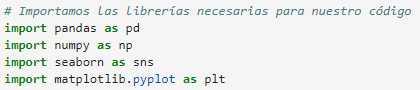
\includegraphics[scale = 0.7]{import.png}
\end{center}

Leemos el archivo de manera un poco diferente a la que hemos estado usando:

\begin{center}
    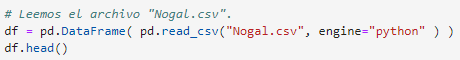
\includegraphics[scale = 0.7]{read.png}
\end{center}

Eliminamos las columnas con datos nulos, para mejor manejo del DataFrame.

\begin{center}
    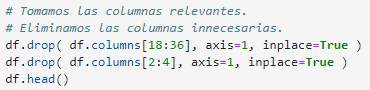
\includegraphics[scale = 0.7]{unnamed.png}
\end{center}
\clearpage

Creamos una nueva columna \textsc{Fecha} a partir de las columnas de \textsc{DATE} y \textsc{TIME}:

\begin{center}
    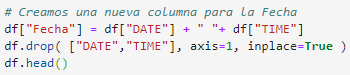
\includegraphics[scale = 0.7]{Fecha.png}
\end{center}

Cambiamos el tipo de datos a float para poder manejar los números y operar con ellos.

\begin{center}
    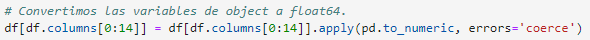
\includegraphics[scale = 0.7]{float.png}
\end{center}

Usamos la función de \textit{corr()} para encontrar la correlación entre variables en una matriz:
\begin{center}
    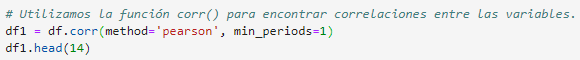
\includegraphics[scale = 0.7]{corr.png}
\end{center}

Generamos dos Heatmaps con los resultados de las correlaciones para comparando el de Matplotlib y el de Seaborn.

También nos fijamos en los datos donde la correlación es mayor a 0.6
y generamos las gráficas de dispersión para estas.

\section{Resultados}
En las siguientes figuras se muestran los heatmap generados con Seaborn y Matplotlib en ese orden:

\begin{center}
    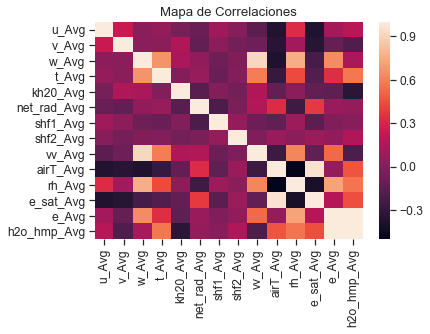
\includegraphics[scale = 0.5]{HmSns.png} 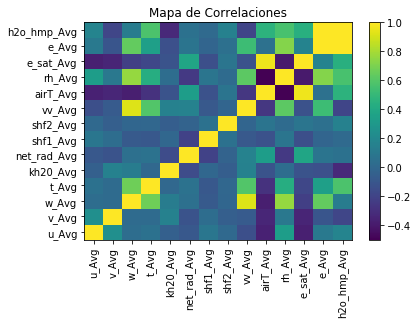
\includegraphics[scale = 0.5]{HmMatplot1.png}
\end{center}

La primera diferencia que vemos es que necesitamos poner manualmente los nombres al eje X y eje Y, también se puede poner manualmente la barra de colores que nos indica el valor de cada color aproximado.

Se obtuvieron muchas gráficas donde la correlación es mayor a 0.6, en seguida se muestran las gráficas generadas.

\begin{center}
    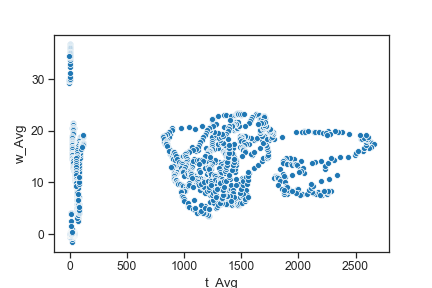
\includegraphics[scale = 0.5]{corr1.png}
    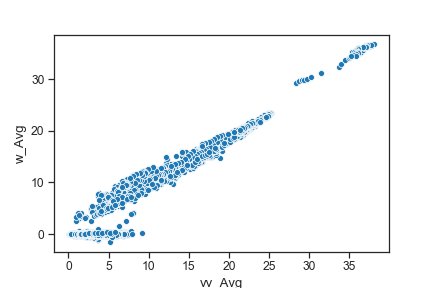
\includegraphics[scale = 0.5]{corr2.png}
    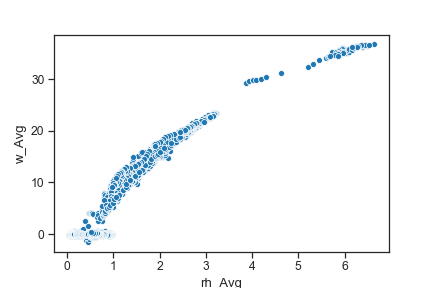
\includegraphics[scale = 0.5]{corr3.png}
    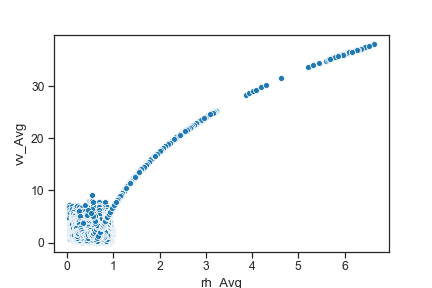
\includegraphics[scale = 0.5]{corr4.png}
    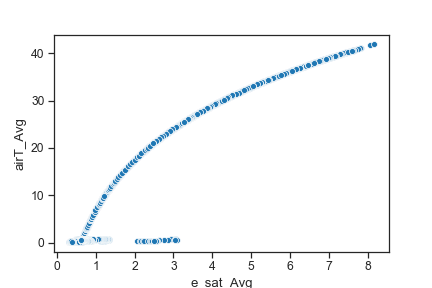
\includegraphics[scale = 0.5]{corr5.png}
    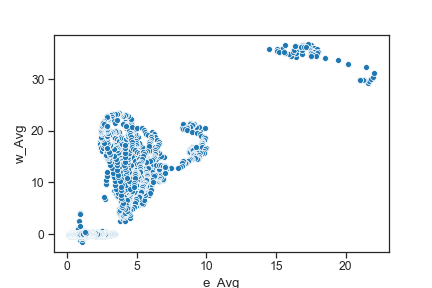
\includegraphics[scale = 0.5]{corr6.png}
    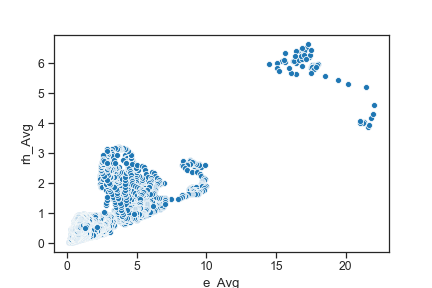
\includegraphics[scale = 0.5]{corr7.png}
\end{center}

\clearpage

En la siguiente, la correlación es muy cercana a 1 por lo tanto la gráfica será aproximadamente lineal.

\begin{center}
    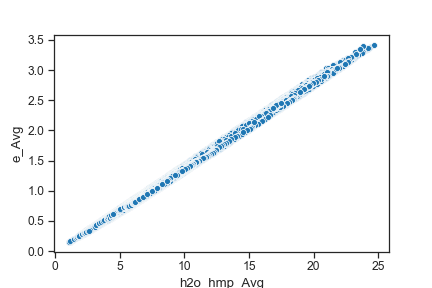
\includegraphics[scale = 0.5]{corr8.png}
\end{center}

\section{Conclusión}
En Seaborn las gráficas se vuelven una tarea mucho más sencilla que con matplotlib, ya trae implícita algunas funciones que en cambio con matplotlib lo tienes que introducir manualmente lo que nos quita tiempo y además hace más lento el proceso de la lectura del código y generación de gráficas.

En cuanto a las gráficas que se generaron en esta actividad, la correlación nos muestra que tan parecidos o relacionados están ciertos valores, en este caso encontramos que sólo una gráfica tenía una correlación lineal.

\section{Bibliografía}
\begin{itemize}
    \item Seaborn: statistical data visualization. (2018). Consultado el 20 de Marzo del 2019, de Seaborn. Sitio web: 
    
    https://seaborn.pydata.org/
    
    \item Probabilidad y Estadística con Python (2015). Consultado el 24 de Marzo del 2019, de Raul E. Lopez Briega Matemáticas, análisis de datos y python. Sitio web:
    
    https://relopezbriega.github.io/blog/2015/06/27/probabilidad-y-estadistica-con-python/
    
    \item 
    
\end{itemize}


\end{document}
